\documentclass[xcolor={svgnames}]{beamer}
\usetheme[
numbering=fraction, % curr_page / total_page
block=fill,         % 为 block 显示方框
% progressbar=frametitle % add a progressbar at frametitle
sectionpage=progressbar
]{metropolis}

%% 保留熟悉的数学字体:两种方法
% \usefonttheme[onlymath]{serif}
\renewcommand\mathfamilydefault{\rmdefault}


\input ../defs.tex  % some frequently used alias


\usepackage[english]{babel}
% \usepackage{enumitem} % 支持自定义 item symbol
\usepackage{tikz}
\usetikzlibrary{tikzmark,positioning,shapes,calc}
\usepackage{mathtools}
\usepackage{amsmath}
\usepackage{fancybox} %支持文本框
\usepackage{subfig} %支持subfig
\usepackage{cite}
%\usepackage{biblatex}
%\usepackage[backend=biber,style=numeric-comp,sorting=none]{biblatex}
%\addbibresource{int-ref.bib}

% Removes icon in bibliography
\setbeamertemplate{bibliography item}[text]

% add following for otherwise it will complain
% see https://tex.stackexchange.com/questions/426088/texlive-pretest-2018-beamer-and-subfig-collide
\makeatletter
\let\@@magyar@captionfix\relax
\makeatother
%%%

%=== font customization ===%
%%
%% Note that once use customizing fonts, switch to xelatex
%%
% \usepackage{fontenc}
% \setsansfont{Varela Round}
% % \setsansfont{IM FELL DW Pica}
% \setmonofont{DejaVu Sans Mono}
% \setmathfont{Fira Sans}


% % 目录标数字
\setbeamertemplate{section in toc}[sections numbered]
% % 无序列表用实心点
% \setbeamertemplate{itemize item}{$\bullet$}
% \setbeamertemplate{navigation symnols}{}

%% 设置列表的 item symbol
% \setbeamertemplate{itemize item}{\textbullet}
% \setbeamertemplate{itemize subitem}{$\blacktriangleright$}
% \setbeamertemplate{itemize subsubitem}{$\checkmark$}

%% 定理环境计数
\setbeamertemplate{theorems}[numbered]
% \setbeamertemplate{lemmas}[numbered]

% 定义颜色
\definecolor{alizarin}{rgb}{0.82, 0.1, 0.26} % 红色
\definecolor{DarkFern}{HTML}{407428}         % 绿色
\definecolor{tyorange}{HTML}{ff6600}
\definecolor{tyblue}{HTML}{0066ff}
\colorlet{main}{DarkFern!100!white}          % 第一种设置方法
\colorlet{main}{red!70!black}                % 第二种设置方法
\definecolor{bistre}{rgb}{0.24, 0.17, 0.12}  % 黑色
\definecolor{mygrey}{rgb}{0.52, 0.52, 0.51}  % 灰色
\colorlet{main}{tyblue}
\colorlet{text}{bistre!100!white}

% 不同元素指定不同颜色,fg是本身颜色,bg是背景颜色,!num!改变数值提供渐变色
% \setbeamercolor{title}{fg=main}
% \setbeamercolor{frametitle}{fg=main}
% \setbeamercolor{section in toc}{fg=text}
% \setbeamercolor{normal text}{fg=text}
% \setbeamercolor{block title}{fg=alizarin,bg=mygrey!20!white}
% \setbeamercolor{block body}{fg=black,bg=mygrey!15!white}
% \setbeamercolor{qed symbol}{fg=main} % 证明结束后的框颜色
% \setbeamercolor{math text}{fg=black}

%=== set theme background color to white ===%
% \setbeamercolor{background}{bg=black}
\setbeamercolor{alerted text}{fg=red!50!black}
\setbeamercolor{normal text}{fg=black!85!}
\setbeamercolor{example text}{fg=black!50!cyan}
% \setbeamercolor{frametitle}{bg=Grey}



%-------------------正文-------------------------%

\title{Elastic InfoGAN}
\subtitle{(draft)}
\author{Bingbing Hu}
\institute{SIST, ShanghaiTech}
\date{\today}

\begin{document}

\frame[plain,noframenumbering]{\titlepage}

%=== index page ===%
\begin{frame}{Outline}
\tableofcontents
\end{frame}

%=== begin your slides ==%
\section{Intro}
% 生成当前 section 的 outline page
% \frame{\frametitle{Outline}\tableofcontents[currentsection]}
 
%%%%%%%%%%%%%%%%%%%%%%%%%%%%%%%%%%%%%%%%%%%%%%%%%%%%%%%%%%%%%

\begin{frame}
  Elastic-InfoGAN learns to disentangle object identity from other low-level 
  aspects in class-imbalanced datasets.

  Experiments show that
  \begin{itemize}
    \item better disentanglement of object identity;
    \item better approximation of class imbalance in the data.
  \end{itemize}
\end{frame}

%%%%%%%%%%%%%%%%%%%%%%%%%%%%%%%%%%%%%%%%%%%%%%%%%%%%%%%%%%%%%

\begin{frame}
  \begin{figure}[p]
    \centering
    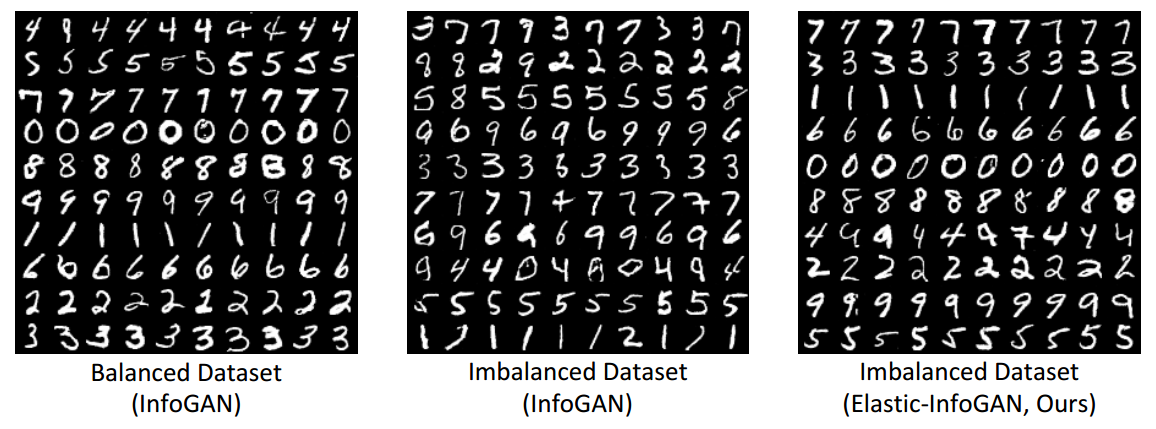
\includegraphics[width=1.0\textwidth]{figures/triple-compare.png}
    \caption{A comparison of results.}
    \label{fig:1}
  \end{figure}
\end{frame}

%%%%%%%%%%%%%%%%%%%%%%%%%%%%%%%%%%%%%%%%%%%%%%%%%%%%%%%%%%%%%

\begin{frame}
  There are literatures that deal with disentangled representation learning,
  also learning from imbalanced data. But we do the both!

  In other words, we do \alert{generative}, \alert{disentangled} representation
  learning in a \alert{unsupervised} setting based on \alert{imbalanced} data.
\end{frame}

%%%%%%%%%%%%%%%%%%%%%%%%%%%%%%%%%%%%%%%%%%%%%%%%%%%%%%%%%%%%%

\section{Problem Formulating}
\begin{frame}
  $N$ unlabeled images from $k$ different classes:
  \[
    \mathcal{X} = \{x_1, \cdots, x_N\}
  \]

  Our goal:
  \begin{itemize}
    \item Learn a generative model $G$ that can disentangle \emph{object category}
      from other aspects;
    \item recover the data distribution (maybe imbalanced).
  \end{itemize}
\end{frame}

%%%%%%%%%%%%%%%%%%%%%%%%%%%%%%%%%%%%%%%%%%%%%%%%%%%%%%%%%%%%%

\begin{frame}
  Recall of InfoGAN,
  \[
  \begin{split}
    \min_{G,Q} \max_D V_{\text{InfoGAN}}(D, G, Q) &= 
    V_{\text{GAN}}(D,G) - \lambda_1 L_1(G,Q) \\
        L_1(G,Q) &= \E_{c\sim P(c), x\sim G(z,c)}[\log Q(c|x)] + H(c)
  \end{split}
  \]
\end{frame}

%%%%%%%%%%%%%%%%%%%%%%%%%%%%%%%%%%%%%%%%%%%%%%%%%%%%%%%%%%%%%

\begin{frame}{Elastic InfoGAN}
  Two augmentations to InfoGAN,
  \begin{enumerate}
    \item learning the prori distribution,
    \item learning object identities.
  \end{enumerate}
  \only<2>{
    For the 2nd, we enforce \emph{identity-preserving transformation} invariance 
    in the learned latent variables so that the resulting disentanglement 
    favors groups that coincide with object identities.
  }
\end{frame}

%%%%%%%%%%%%%%%%%%%%%%%%%%%%%%%%%%%%%%%%%%%%%%%%%%%%%%%%%%%%%

\begin{frame}{Learning prori distribution}
  Replace fixed categorical distribution by Gumbel-Softmax distribution. For a
  categorical distribution $(p_1, \cdots, p_k)$, sample $k$-dimensional vector
  $\bd{c}$ where
  \[
    c_i = \frac{\exp((\log(p_i) + g_i) / \tau)}
    {\sum_{j=1}^k \exp((\log(p_j) + g_j) / \tau)}
    \quad \text{for } i = 1, \dots, k.
  \]

  \begin{itemize}
    \item $g_i, g_j$: samples from $Gumbel(0,1)$,
    \item $\tau$: softmax temperature, controls the degree to which samples 
      from Gumbel-Softmax resemble the categorical distribution.
  \end{itemize}
\end{frame}

%%%%%%%%%%%%%%%%%%%%%%%%%%%%%%%%%%%%%%%%%%%%%%%%%%%%%%%%%%%%%

\begin{frame}{Learning prori distribution}
  This should be enough to handle the imbalance, once the true imbalance gets
  reflected in the class probabilities, the category code should disentangle
  object category. But experiments don't show that well!
  
  \begin{figure}[hp]
    \centering
    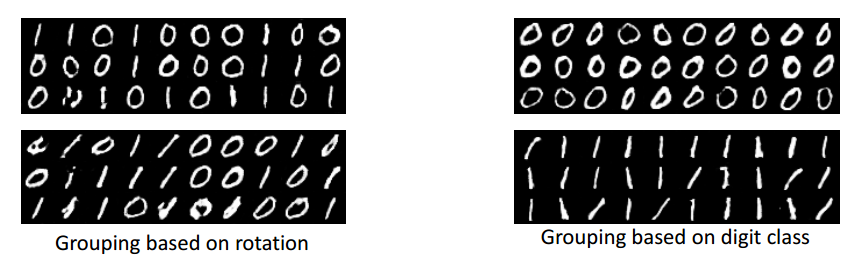
\includegraphics[width=0.9\textwidth]{figures/disentangle.png}
    \caption{Unsupervised grouping can focus on non-categorical attributes 
    such as rotation of the digit.}
    \label{fig:dis}
  \end{figure}

\end{frame}

%%%%%%%%%%%%%%%%%%%%%%%%%%%%%%%%%%%%%%%%%%%%%%%%%%%%%%%%%%%%%

\begin{frame}{Learning object identities}
  Here comes the second augmentation: \alert{learning object identities}. 

  We want our model
  \begin{itemize}
    \item focus on high level object identity,
    \item invariant to low level factors (rotation, thickness, etc.).
  \end{itemize}
\end{frame}

%%%%%%%%%%%%%%%%%%%%%%%%%%%%%%%%%%%%%%%%%%%%%%%%%%%%%%%%%%%%%

\begin{frame}{What we do}
  For any real image $x \sim P_{\text{data}}(x)$, we apply a set of
  transformations $\delta$ to obtain a transformed image $x' = \delta(x)$.
  Then we introduce a loss
  \[
    L_{\text{trans}}(Q) = \mathsf{d}(Q(c_x | x), Q(c_{x'} | x')),
  \]
  where $\mathsf{d}(\cdot)$ is a distance metric.

  Note that
  \begin{itemize}
    \item these transformations are not learned,
    \item the object identity won't change after these transformations under
      a human view.
  \end{itemize}
\end{frame}

%%%%%%%%%%%%%%%%%%%%%%%%%%%%%%%%%%%%%%%%%%%%%%%%%%%%%%%%%%%%%

\begin{frame}{One more thing}
  $Q(c|x)$ should have low entropy (peaky class distribution) either for
  $x \sim P_{\text{data}}$ or $\tilde{x} \sim P_G$.

  \begin{itemize}
    \item For $\tilde{x} \sim P_G$, this is ensured by InfoGAN framework.
    \item For real images $x \sim P_{\text{data}}$, $L_{\text{trans}}$ isn't
      sufficient to ensure this.
  \end{itemize}
  We hence add an additional entropy loss which forces $c_x$ and $c_{x'}$ to 
  have low entropy (s) class distributions:
  \[
    L_{\text{ent}}(Q) = \mathsf{s}(Q(c_x | x)) + \mathsf{s}(Q(c_{x'} | x')).
  \]
\end{frame}

%%%%%%%%%%%%%%%%%%%%%%%%%%%%%%%%%%%%%%%%%%%%%%%%%%%%%%%%%%%%%

\begin{frame}
  The whole loss becomes
  \[
    \begin{split}
      \min_{G, Q}\max_D L_{\text{final}} &= V_{\text{InfoGAN}}(D, G, Q) + 
      \lambda_2 L_{\text{trans}}(Q) + \lambda_3 L_{\text{ent}}(Q) \\
      V_{\text{InfoGAN}}(D, G, Q) &= 
      V_{\text{GAN}}(D,G) - \lambda_1 L_1(G,Q).
    \end{split}
  \]
  
  \begin{itemize}
    \item $V_{\text{InfoGAN}}$ plays the role of generating realistic images 
      and associating the latent variables to correspond to some factor of 
      variation in the data, 
    \item $L_{\text{trans}}$ will push the discovered factor of variation to 
      be close to object identity,
    \item $L_{\text{ent}}$ ensures $Q$ behaves similarly for real and fake 
      image distributions.
  \end{itemize}
\end{frame}

%%%%%%%%%%%%%%%%%%%%%%%%%%%%%%%%%%%%%%%%%%%%%%%%%%%%%%%%%%%%%

\begin{frame}
  The whole architecture looks like this:
  \begin{figure}[hbp]
    \centering
    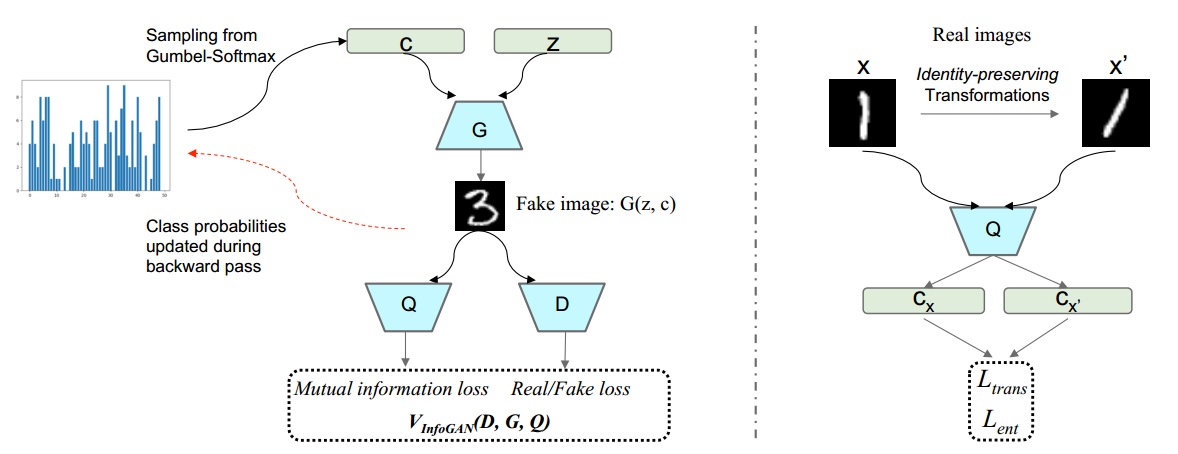
\includegraphics[width=\textwidth]{figures/arch.png}
    \caption{Elastic InfoGAN architecture.}
    \label{fig:arch}
  \end{figure}
\end{frame}

%%%%%%%%%%%%%%%%%%%%%%%%%%%%%%%%%%%%%%%%%%%%%%%%%%%%%%%%%%%%%

\section{Experiments}
\begin{frame}{Baselines and evaluation metric}
  Different settings:
  \begin{itemize}
    \item \emph{Uniform InfoGAN}: fixed and uniform categorical distribution.
    \item \emph{Ground-truth InfoGAN}: fixed, imbalanced categorical 
      distribution that reflect the true imbalance.
    \item \emph{Ground-truth InfoGAN + Transformation constraint}: ditto but
      add $L_{\text{trans}}$.
    \item \emph{Gumbel-softmax}: learnable categorical distribution.
    \item \emph{Gumbel-softmax + Transformation constraint}: ditto but add 
      $L_{\text{trans}}$.
    \item \emph{Gumbel-softmax + Transformation constraint + Entropy loss 
      (Elastic-InfoGAN)}: ditto but add $L_{\text{ent}}$.
    \item \emph{JointVAE}: another paper.
  \end{itemize}
\end{frame}

%%%%%%%%%%%%%%%%%%%%%%%%%%%%%%%%%%%%%%%%%%%%%%%%%%%%%%%%%%%%%

\begin{frame}{Baselines and evaluation metric}
  Evaluation metrics:
  \begin{itemize}
    \item \emph{Average entropy}
    \item \emph{Normalized Mutual Information}
    \item \emph{Root Mean Square Error}
  \end{itemize}

  More on paper\ldots
\end{frame}

%%%%%%%%%%%%%%%%%%%%%%%%%%%%%%%%%%%%%%%%%%%%%%%%%%%%%%%%%%%%%

% Here comes the bibliography.
% \begin{frame}[allowframebreaks]{References}
% 	%\bibliographystyle{plain}
% 	%\bibliography{int-ref}
% 	\bibliographystyle{amsalpha}
% 	\bibliography{./int-ref.bib}
% \end{frame}

%%%%%%%%%%%%%%%%%%%%%%%%%%%%%%%%%%%%%%%%%%%%%%%%%%%%%%%%%%%%%

\begin{frame}[standout]
  \Huge Thank you!
\end{frame}

% \begin{frame}[label=conclusion, standout]{Conclusion}
%   Awesome slide
% \end{frame}
\end{document}
